%====================================================================
%
%								Packages
%
%====================================================================
\documentclass[12pt , a4paper]{article}						   
\usepackage[left=2cm, right=2cm, top=2.5cm, bottom=2.5cm]{geometry}
\usepackage{fancyhdr , lipsum}
\usepackage{mathptmx}
\usepackage{anyfontsize}
\usepackage{t1enc}
\usepackage{csquotes}
\usepackage{blindtext}
\usepackage{enumitem}
\usepackage{xcolor}
\usepackage[linktocpage]{hyperref}
\usepackage{graphicx}
\usepackage{float}
\usepackage{subcaption}
\usepackage[section]{placeins} 
\usepackage[T1]{fontenc}
\usepackage{fontspec}
\usepackage{tcolorbox}
\usepackage[english]{babel}
\usepackage[export]{adjustbox}
\usepackage{amsmath}
\usepackage{stmaryrd} % used for arrows
%====================================================================
%
%								Defined Colors
%
%====================================================================
% http://latexcolor.com/
\usepackage{color}
\definecolor{lightGrey}{rgb}{105,105,105}
\definecolor{azure}{rgb}{0.94, 1.0, 1.0}
\definecolor{black}{rgb}{0,0,0}
\definecolor{babyblue}{rgb}{0.54, 0.81, 0.94}
\definecolor{aureolin}{rgb}{0.99, 0.93, 0.0}
\definecolor{bananamania}{rgb}{0.98, 0.91, 0.71}
\definecolor{bazaar}{rgb}{0.6, 0.47, 0.48}
\definecolor{blizzardblue}{rgb}{0.67, 0.9, 0.93}
\definecolor{bubblegum}{rgb}{0.99, 0.76, 0.8}
\definecolor{byzantium}{rgb}{0.44, 0.16, 0.39}
\definecolor{capri}{rgb}{0.0, 0.75, 1.0}
\definecolor{charcoal}{rgb}{0.21, 0.27, 0.31}
\definecolor{coolblack}{rgb}{0.0, 0.18, 0.39}
\definecolor{cream}{rgb}{1.0, 0.99, 0.82}
\definecolor{Midnightblue}{RGB}{34,34,103}
%====================================================================
%
%								Code Highlighter Package
%
%====================================================================
% Include this package if not already included: \usepackage{color}
\usepackage[T1]{fontenc}
\usepackage{inconsolata}
\usepackage{listings}
\definecolor{pblue}{rgb}{0.13,0.13,1}
\definecolor{pgreen}{rgb}{0,0.5,0}
\definecolor{pred}{rgb}{0.9,0,0}
\definecolor{pgrey}{rgb}{0.46,0.45,0.48}
\definecolor{background}{RGB}{39, 40, 34}
\definecolor{string}{RGB}{230, 219, 116}
\definecolor{comment}{RGB}{117, 113, 94}
\definecolor{normal}{RGB}{248, 248, 242}
\definecolor{identifier}{RGB}{166, 226, 46}

\definecolor{mygray}{rgb}{0.4,0.4,0.4}
\definecolor{mygreen}{rgb}{0,0.8,0.6}
\definecolor{myorange}{rgb}{1.0,0.4,0}
\definecolor{includeColor}{RGB}{197,134,192}
\definecolor{myblue}{RGB}{86,156,214}


\definecolor{background}{RGB}{39, 40, 34}
\definecolor{string}{RGB}{230, 219, 116}
\definecolor{comment}{RGB}{117, 113, 94}
\definecolor{normal}{RGB}{248, 248, 242}
\definecolor{identifier}{RGB}{166, 226, 46}

\lstset{
  language=Java,   
 commentstyle=\color{mygreen},             			% choose the language of the code
  numbers=left,                   		% where to put the line-numbers
  stepnumber=1,                   		% the step between two line-numbers.        
  numbersep=5pt,                  		% how far the line-numbers are from the code
  numberstyle=\tiny\color{black}\ttfamily,
  backgroundcolor=\color{background},  		% choose the background color. You must add \usepackage{color}
  showspaces=false,               		% show spaces adding particular underscores
  showstringspaces=false,         		% underline spaces within strings
  showtabs=false,                 		% show tabs within strings adding particular underscores
  tabsize=4,                      		% sets default tabsize to 2 spaces
  captionpos=b,                   		% sets the caption-position to bottom
  breaklines=true,                		% sets automatic line breaking
  breakatwhitespace=true,         		% sets if automatic breaks should only happen at whitespace
  title=\lstname,                 		% show the filename of files included with \lstinputlisting;
  basicstyle=\color{normal}\ttfamily,					% sets font style for the code
  keywordstyle=\color{myblue},	% sets color for keywords
  stringstyle=\color{string}\ttfamily,		% sets color for strings
  emph={format_string, eff_ana_bf, permute, eff_ana_btr},
  emphstyle=\color{identifier}\ttfamily,
}



\lstset{
  emph = {include, String, StringBuilder},
  emphstyle = \color{includeColor}
}

%\begin{lstlisting}[language=java]
%\end{lstlisting}

%====================================================================
%
%								Output Box
%
%====================================================================

%\begin{tcolorbox}
%\textbf{Output:}\\
%>> g++ -o program main.cpp\\
%\end{tcolorbox}

%% Custom TcolorBox 


%%%%%%%%%% Sample Box %%%%%%%%%%%%%%%%
\newtcolorbox{BoxName}[3][]
{
  colframe = #2!25,
  colback  = #2!10,
  coltitle = #2!20!black,  
  title    = {#3},
  #1,
}

%%%%%%%%%% Important Box %%%%%%%%%%%%%%%%
\definecolor{imp_box_green_title}{RGB}{191,254,192}
\definecolor{imp_box_green_bg}{RGB}{230,255,230}
\definecolor{imp_box_blue_title}{RGB}{0,0,139}

\newtcolorbox{importantBox}[1][]
{
  colframe = {imp_box_green_title},
  colback  = {imp_box_green_bg},
  coltitle = {imp_box_green_title},  
  title    = {\textcolor{imp_box_blue_title}{\textbf{Attention}}},
  #1,
}

%%%%%%%%%% Problem Definition Box %%%%%%%%%%%%%%%%
\definecolor{prob_box_white_title}{RGB}{145,81,23}
\definecolor{prob_box_chocolate_bg}{RGB}{210,105,30}
\definecolor{prob_box_white_text}{RGB}{255,255,255}
\definecolor{prob_box_paleGreen_text}{RGB}{245,245,220}

\definecolor{google_logo_color_blue}{RGB}{66, 133, 244}
\definecolor{google_logo_color_red}{RGB}{219, 68, 55}
\definecolor{google_logo_color_yellow}{RGB}{244, 180, 0}
\definecolor{google_logo_color_green}{RGB}{15, 157, 88}

\newtcolorbox{problemDefBox}[1][]
{
  colframe = {prob_box_white_title},
  colback  = {prob_box_chocolate_bg},
  coltitle = {prob_box_white_title},  
 coltext={prob_box_paleGreen_text},
  title    = {\textcolor{prob_box_white_text}{\textbf{Problem}}},
  #1,
}
%====================================================================
%
%								Text Highlighter Package
%
%====================================================================
\usepackage{xcolor}
%\colorbox{pink}{highlight}
%\newcommand{\hl}[1]{\colorbox{coolblack}{\color{cream}\textbf{#1}\color{black}}}
%====================================================================
%
%								Some Useful Tips
%
%====================================================================

%***********************************
%			Items
%***********************************

%\begin{itemize}
%\item \\[7pt]
%\end{itemize}

%====================================================================
%
%								Variables
%
%====================================================================
%\newcommand{}[1]{}
\newcommand{\dateOfWritingThisBooklet}{July 2021}
\newcommand{\hl}[1]{\colorbox{coolblack}{\color{cream}\textbf{#1}\color{black}}}
\newcommand{\bs}{$\backslash$}
\newcommand{\arrow}{$\shortrightarrow$}
\newcommand{\google}{\href{https://www.google.com/}{\color{google_logo_color_blue}G\color{google_logo_color_red}o\color{google_logo_color_yellow}o\color{google_logo_color_blue}g\color{google_logo_color_green}l\color{google_logo_color_red}e\color{black}} \. }


%====================================================================
%
%								Header / Footer
%
%====================================================================
\renewcommand{\footrulewidth}{0.4pt}% default is 0pt
\pagestyle{fancy}
\fancyhf{}
\chead{}
\rhead{}
\lhead{Programming In Java}
\cfoot{Page \thepage}
\lfoot{Vrije Universiteit Brussel}
\rfoot{October 2021-22}
%====================================================================
%
%								Start of The Document
%
%====================================================================
%====================================================================
%====================================================================
%====================================================================
%====================================================================
%====================================================================
%====================================================================
%====================================================================
%====================================================================
%====================================================================
%====================================================================
%====================================================================
%====================================================================
%====================================================================
%====================================================================
%====================================================================
%====================================================================
%====================================================================
%====================================================================
%====================================================================
%====================================================================
%====================================================================
%====================================================================
%====================================================================
%====================================================================
%====================================================================
%====================================================================
%====================================================================
%====================================================================
%====================================================================
%====================================================================
%====================================================================
%====================================================================
%====================================================================
%====================================================================
%====================================================================
%====================================================================
%====================================================================
%====================================================================
%====================================================================
%====================================================================
%====================================================================
%====================================================================

\begin{document}
%====================================================================
%
%								First Page (Author, ...)
%
%====================================================================
\thispagestyle{empty}
 \begin{center}

{
\centering
\fontfamily{titr}  
\fontsize{20pt}{20pt}
\selectfont 
In The Name Of God
}
\\[60pt]
 %picture
\begin{figure}[H]
\centering

\includegraphics[width=0.4\textwidth]{VUB_Logo.jpg}
\caption*{}
\label{f-0-0}
\end{figure}
{
\centering
\fontfamily{titr}  
\fontsize{18pt}{18pt}
\selectfont 
Programming In Java
}
\\[20pt]
{
\centering
\fontfamily{titr}  
\fontsize{16pt}{16pt}
\selectfont 
Assignment 2
}
\\[20pt]
{
\centering
\fontfamily{titr}  
\fontsize{12pt}{12pt}
\selectfont 
\begin{tabular}{r l}
Professor:			&	Dr. Lesley De Cruz\\[5pt]
TA:				&	Hossein Dehghanipour\\[5pt]

\end{tabular}
}
\\[20pt]
{
\centering
\fontfamily{titr}  
\fontsize{12pt}{12pt}
\selectfont 
October 2021
}

\end{center}
 

 
\setmainfont{Times New Roman}
\newpage

%====================================================================
%
%								Table of Content
%
%====================================================================
\tableofcontents
\newpage

%====================================================================
%
%								Section: Basic Syntax
%
%====================================================================
\section{Basic Syntax}

	%======================================
	%
	%	Subsection: Question 1
	%
	%======================================
	\subsection{Print Name}
Write a piece of code in the \textbf{main()} function that gets two inputs from the user \textbf{(firstName, lastName)} and prints them together like the following example:
 

	%--------------------------------------------------------------------%
	%											%
	%				Code Output					%
	%											%
	%--------------------------------------------------------------------%
	\begin{tcolorbox}
	\textbf{Output:}\\
	> Enter your first name:\\
	> Alex\\
	> Enter your last name:\\
	> Adams\\
	> Welcome to MACS, Alex Adams.
	\end{tcolorbox}

	%--------------------------------------------------------------------%
	%											%
	%				Sample Code					%
	%											%
	%--------------------------------------------------------------------%
	\begin{lstlisting}[language=Java]
	public class Main{

	     public static void main(String[] args){
	        // Write your code here
		System.out.println("Enter your first name:");
		String firstName = // Your Code Goes Here 
		System.out.println("Enter your last name:");
		String lastName = //Your Code Goes Here
		System.out.println("Welcome to MACS," + firstName + " " + lastName);
	     }
	}
	\end{lstlisting}


	%======================================
	%
	%	Subsection: Question 2
	%
	%======================================
	\newpage
	\subsection{Calculate Summation}
Write a method named \textbf{int calculateSum(int number)} which gets a \hl{number} as its input argument and adds all of the numbers from \textbf{zero} to the given \textbf{number} and prints the result.
	%--------------------------------------------------------------------%
	%											%
	%				Code Output					%
	%											%
	%--------------------------------------------------------------------%
	\begin{tcolorbox}
	\textbf{Example:}\\
	calculateSum(5) -> 15 (0 + 1 + 2 + 3 + 4 + 5)\\
	calculateSum (10) -> 55 (0 + 1 + 2 + ... + 10)
	\end{tcolorbox}

	%--------------------------------------------------------------------%
	%											%
	%				Sample Code					%
	%											%
	%--------------------------------------------------------------------%
	\begin{lstlisting}[language=Java]
	public class Main{
		public static int caculateSum( int number ){
			int sum = 0 ;
			// Your Code Goes Here

			// Your Code Ends Here
			return sum;
		}
	     public static void main(String[] args){
			System.out.println(calculateSum(5)) ;
			System.out.println(calculateSum(10)) ;
	     }
	}
	\end{lstlisting}

	%======================================
	%
	%	Subsection: Question 3
	%
	%======================================
	\newpage
	\subsection{Calculate Summation II}
	Modify the previous function \textbf{int calculateSum (int lowerBound, int upperBound)} in such a way that calculates the summation of numbers between the \textbf{lowerBound} and \textbf{upperBound}.\\
	%--------------------------------------------------------------------%
	%											%
	%				Important Box					%
	%											%
	%--------------------------------------------------------------------%

	\begin{importantBox}

		\begin{itemize}
			\item  Please be aware that the method returns \textbf{-1} as an error if the lower bound was larger than the upper bound (lowerBound > upperBound).
		\end{itemize}
	\end{importantBox}


	%--------------------------------------------------------------------%
	%											%
	%				Sample Code					%
	%											%
	%--------------------------------------------------------------------%
	\begin{lstlisting}[language=Java]
public class Main{
	public static int calculateSum(int lowerBound, int upperBound){
		int sum = 0;
		if(lowerBound < upperBound){
		// Your Code Goes Here

		// Your Code Ends Here
        	}

		else{
			sum = -1;
		}
		return (int)sum;
	}
}
	public static void main(String[] args){
		System.out.println(calculateSum(5, 10)) ;
		System.out.println(calculateSum(5, 2)) ;
	}
}
	\end{lstlisting}

	%--------------------------------------------------------------------%
	%											%
	%				Code Output					%
	%											%
	%--------------------------------------------------------------------%
	\begin{tcolorbox}
	\textbf{Output:}\\
	 > 45 -> (5 + 6 + 7 + 8 + 9 + 10) \\
	 > -1\\
	\end{tcolorbox}

	%======================================
	%
	%	Subsection: Question 4
	%
	%======================================
	\newpage
	\subsection{Vertical Pyramid}
Write a method that gets an integer input as parameter and based on the number prints the following pattern:
	%--------------------------------------------------------------------%
	%											%
	%				Sample Code					%
	%											%
	%--------------------------------------------------------------------%
	\begin{lstlisting}[language=Java]
public class Main{
	public static void printPyramid(int number){
		// Your Code Goes Here

		// Your Code Ends Here
	}
}
	public static void main(String[] args){
		printPyramid(5);
	}
}
	\end{lstlisting}

	%--------------------------------------------------------------------%
	%											%
	%				Code Output					%
	%											%
	%--------------------------------------------------------------------%
	\begin{tcolorbox}
	\textbf{Output:}\\
	+\\
	++\\
	+++\\
	++++\\
	+++++\\
	++++\\
	+++\\
	++\\
	+
	\end{tcolorbox}

	%======================================
	%
	%	Subsection: Question 5
	%
	%======================================
	\newpage
	\subsection{Diamond}
Write a method that gets an integer and a character as input parameters and based on them prints the following pattern:
	%--------------------------------------------------------------------%
	%											%
	%				Sample Code					%
	%											%
	%--------------------------------------------------------------------%
	\begin{lstlisting}[language=Java]
public class Main{
	public static void printDiamond(int number, char symbol){
		// Your Code Goes Here

		// Your Code Ends Here
	}
}
	public static void main(String[] args){
		printDiamond(10, '*');
		printDiamond(12, '.')
	}
}
	\end{lstlisting}

	%--------------------------------------------------------------------%
	%											%
	%				Code Output					%
	%											%
	%--------------------------------------------------------------------%
	\begin{tcolorbox}
	\textbf{Output:}\\
%picture
\begin{figure}[H]
\centering
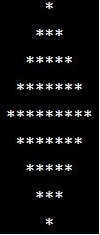
\includegraphics[width=0.2\textwidth]{5-1.jpg}
\caption*{}
\label{f-0-0}
\end{figure}
%
%picture
\begin{figure}[H]
\centering
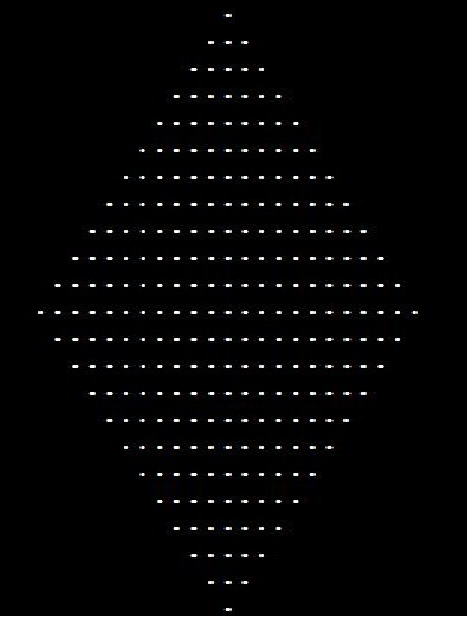
\includegraphics[width=0.4\textwidth]{5-2.jpg}
\caption*{}
\label{f-0-0}
\end{figure}
	\end{tcolorbox}



	%======================================
	%
	%	Subsection: Question 6
	%
	%======================================
	\newpage
	\subsection{Remove Character Occurrences}
Write a method called \textbf{public static String removeOccurences(String sentence, char c)} that removes all of the occurrences of a character inside a String and returns the remaining sentence.\\
	%--------------------------------------------------------------------%
	%											%
	%				Important Box					%
	%											%
	%--------------------------------------------------------------------%

	\begin{importantBox}

		\begin{itemize}
			\item Please search about a class called \href{https://docs.oracle.com/javase/tutorial/java/data/buffers.html}{"String Builder"} before proceeding to solve the problem.  
		\end{itemize}
	\end{importantBox}

	%--------------------------------------------------------------------%
	%											%
	%				Sample Code					%
	%											%
	%--------------------------------------------------------------------%
	\begin{lstlisting}[language=Java]
public class Main{
	public static String removeOccurences(String sentence, char c){
		StringBuilder newSentence = new StringBuilder();
		// Your Code Goes Here

		// Your Code Ends Here	
		return newSentence.toString();
	}
}
	public static void main(String[] args){
		removeOccurences("AppliedComputerScience", 'e');
	}
}
	\end{lstlisting}


	%--------------------------------------------------------------------%
	%											%
	%				Code Output					%
	%											%
	%--------------------------------------------------------------------%
	\begin{tcolorbox}
	\textbf{Output:}\\
	ApplidComputrScinc
	\end{tcolorbox}




	%======================================
	%
	%	Subsection: Question 7
	%
	%======================================
	\newpage
	\subsection{Remove Occurrences of Character Array }
Write a method called\textbf{public String removeOccurences(String sentence, char[] characters)} that removes all of the occurrences of the characters inside a String and returns the remaining sentence.\\

	%--------------------------------------------------------------------%
	%											%
	%				Important Box					%
	%											%
	%--------------------------------------------------------------------%

	\begin{importantBox}

		\begin{itemize}
			\item  'T' and 't' are considered totally different characters.
		\end{itemize}
	\end{importantBox}
	%--------------------------------------------------------------------%
	%											%
	%				Sample Code					%
	%											%
	%--------------------------------------------------------------------%
	\begin{lstlisting}[language=Java]
public class Main{
	public static String removeOccurences(String sentence, char[] c){
		StringBuilder newSentence = new StringBuilder();
		// Your Code Goes Here

		// Your Code Ends Here	
		return newSentence.toString();
	}
}
	public static void main(String[] args){
		String modifiedOne = removeOccurences("We Work In The Darkness To Serve The Light", ['t','e']);
		System.out.println(modifiedOne);

		String modifiedTwo = removeOccurences("You are great", ['a']));
		System.out.println(modifiedTwo);
		
		char[] mustBeRemoved = ['A','B','C','D','E','f','g'] ;
		String originalSentence = "ABCDEfghAAA";
		removeOccurences(originalSentence , mustBeRemoved);
	}
}
	\end{lstlisting}


	%--------------------------------------------------------------------%
	%											%
	%				Code Output					%
	%											%
	%--------------------------------------------------------------------%
	\begin{tcolorbox}
	\textbf{Output:}\\
	"W Work In Th Darknss srv Th ligh"\\
	"You re gret"\\
	"h"
	\end{tcolorbox}



	%======================================
	%
	%	Subsection: Question 8
	%
	%======================================
	\newpage
	\subsection{Remove Word Occurrences}
Write a function called \textbf{public static String removeWords(String sentence, String word)} that removes all of the occurrences of the given word inside a String and returns the remaining sentence.

	%--------------------------------------------------------------------%
	%											%
	%				Sample Code					%
	%											%
	%--------------------------------------------------------------------%
	\begin{lstlisting}[language=Java]
public class Main{
	public static String removeWords(String sentence, String word){
		StringBuilder newSentence = new StringBuilder();
		// Your Code Goes Here

		// Your Code Ends Here	
		return newSentence.toString();
	}
}
	public static void main(String[] args){
		String result = removeWords("The Sheeps Ship Cheap Sheets by Ship", "Ship");
		System.out.println(result);
	}
}
	\end{lstlisting}


	%--------------------------------------------------------------------%
	%											%
	%				Code Output					%
	%											%
	%--------------------------------------------------------------------%
	\begin{tcolorbox}
	\textbf{Output:}\\
	"The Sheeps Cheap Sheets by"
	\end{tcolorbox}

%====================================================================
%
%								Section: Intermediate Level
%
%====================================================================
\newpage
\section{Intermediate Level}

	%======================================
	%
	%	Subsection: Question 1
	%
	%======================================
	\subsection{Celsius to Fahrenheit Conversion}
Write a method that gets an integer as a temperature in Celsius and returns its equivalent in Fahrenheit.

	%--------------------------------------------------------------------%
	%											%
	%				Important Box					%
	%											%
	%--------------------------------------------------------------------%

	\begin{importantBox}

		\begin{itemize}
			\item  \textbf{(C° × 9/5) + 32 = F°}
			\item \href{https://www.google.com/search?q=celcius+to+farenheit&oq=celcius&aqs=chrome.0.69i59j69i57j46i10i199i465i512j0i10l6j0i271.1004j0j4&sourceid=chrome&ie=UTF-8}{Online Celsius to Fahrenheit Calculator}
		\end{itemize}
	\end{importantBox}
	%--------------------------------------------------------------------%
	%											%
	%				Sample Code					%
	%											%
	%--------------------------------------------------------------------%
	\begin{lstlisting}[language=Java]
public class Main{
	public static double celsiusToFahrenheit(int cel){
		double fahrenheit = 0 ;
		// Your Code Goes Here

		// Your Code Ends Here	
		return fahrenheit;
	}
}
	public static void main(String[] args){
		double fahrentheitValueOne = celsiusToFahrenheit(5);
		System.out.println(fahrentheitValueOne);

		
		double fahrentheitValueTwo = celsiusToFahrenheit(21);
		System.out.println(fahrentheitValueTwo);		
	}
}
	\end{lstlisting}


	%--------------------------------------------------------------------%
	%											%
	%				Code Output					%
	%											%
	%--------------------------------------------------------------------%
	\begin{tcolorbox}
	\textbf{Output:}\\
	41\\
	69.8
	\end{tcolorbox}

	%======================================
	%
	%	Subsection: Question 
	%
	%======================================
	\newpage
	\subsection{Fibonacci Using Loops}
Write a method that gets an integer as input and calculates the nth Fibonacci number of \textbf {n = input number} using loops.\\
	%--------------------------------------------------------------------%
	%											%
	%				Important Box					%
	%											%
	%--------------------------------------------------------------------%

	\begin{importantBox}

		\begin{itemize}
			\item  fib(0) = 0,fib(1) = 1, and fib(n) = fib(n-1) + fib(n-2) \\
			\item  \href{https://en.wikipedia.org/wiki/Fibonacci_number}{For more info about Fibonacci Series click here}\\
			\item \href{https://www.omnicalculator.com/math/fibonacci}{Online Fibonacci Calculator}\\
			\item Fibonacci Series: 0, 1, 1, 2, 3, 5, 8, 13, 21, 34, ...
		\end{itemize}
	\end{importantBox}
	%--------------------------------------------------------------------%
	%											%
	%				Sample Code					%
	%											%
	%--------------------------------------------------------------------%
	\begin{lstlisting}[language=Java]
public class Main{
	public static int fib(int n){
		int calculatedFib = 0 ;

		if ( n == 0 ){
			return 0;
		}
		
		else if ( n == 1 ){
			return 1;
		}

		else{

			// Your Code Goes Here
			int loopCounter = // Your Code Goes Here ;
			for (int i = 0 ; i < loopCounter ; i++){
	
			
			}
			// Your Code Ends Here	
		}
		return calculatedFib;
	}
}
	public static void main(String[] args){
		System.out.println(fib(0));	
		System.out.println(fib(1));
		System.out.println(fib(2));
		System.out.println(fib(3));	
		System.out.println(fib(5));	
		System.out.println(fib(6));	
		System.out.println(fib(10));		
	}
}
	\end{lstlisting}


	%--------------------------------------------------------------------%
	%											%
	%				Code Output					%
	%											%
	%--------------------------------------------------------------------%
	\begin{tcolorbox}
	\textbf{Output:}\\
	0\\
	1\\
	1\\
	2\\
	5\\
	8 \\
	55\\
	\end{tcolorbox}

	%======================================
	%
	%	Subsection: Question 3
	%
	%======================================
	\newpage
	\subsection{Fibonacci Using Recursion}
Write a method called recursiveFib that calculates the exact same thing in Question 2 but without using loops. (By using only recursion)
	%--------------------------------------------------------------------%
	%											%
	%				Sample Code					%
	%											%
	%--------------------------------------------------------------------%
	\begin{lstlisting}[language=Java]
public class Main{
	public static int recursiveFib(int n){
		int calculatedFib = 0 ;

		if ( n == 0 ){
			return 0;
		}
		
		else if ( n == 1 ){
			return 1;
		}

		else{

			// Your Code Goes Here
			// You should not use any loops in here


			// Your Code Ends Here	
		}
		return calculatedFib;
	}
}
	public static void main(String[] args){
		System.out.println(recursiveFib(0));		
		System.out.println(recursiveFib(10));		
	}
}
	\end{lstlisting}
	%--------------------------------------------------------------------%
	%											%
	%				Code Output					%
	%											%
	%--------------------------------------------------------------------%
	\begin{tcolorbox}
	\textbf{Output:}\\
	0\\
	55\\
	\end{tcolorbox}

	%======================================
	%
	%	Subsection: Question 4
	%
	%======================================
	\newpage
	\subsection{Factorial Using Recursion}
Write function that takes a number and calculates its factorial by using recursion.


``

Example:
- ) -> 5 * 4 * 3 * 2 * 1 = 120
	%--------------------------------------------------------------------%
	%											%
	%				Important Box					%
	%											%
	%--------------------------------------------------------------------%

	\begin{importantBox}

		\begin{itemize}
			\item   Factorial of 0 is 1\\
			\item For negative numbers, the method should return -1 as an error.\\
			\item  n! = n * (n-1) * (n-2) * ... * 1\\
			\item \href{https://www.calculatorsoup.com/calculators/discretemathematics/factorials.php}{Online Factorial Calculator}\\
		\end{itemize}
	\end{importantBox}

	%--------------------------------------------------------------------%
	%											%
	%				Sample Code					%
	%											%
	%--------------------------------------------------------------------%
	\begin{lstlisting}[language=Java]
public class Main{
	public static int calculateFactorial(int n){
		int calculatedFact = 1 ; // Why not zero?

		if ( n == 0 ){
			return 1;
		}
		else if ( n < 0 ){
			return -1;
		}
		else{
			// Your Code Goes Here
			// You should not use any loops in here


			// Your Code Ends Here	
		}
		return calculatedFact;
	}
	public static void main(String[] args){	
		System.out.println(calculateFactorial(5));		
	}
}
	\end{lstlisting}
	%--------------------------------------------------------------------%
	%											%
	%				Code Output					%
	%											%
	%--------------------------------------------------------------------%
	\begin{tcolorbox}
	\textbf{Output:}\\
	120 -> 1 * 2 * 3 * 4 * 5\\
	
	\end{tcolorbox}

	%======================================
	%
	%	Subsection: Question 5
	%
	%======================================
	\newpage
	\subsection{Binary To Decimal Conversion}
	Write a function takes a number in binary and converts it to decimal and returns the calculated value.
	%--------------------------------------------------------------------%
	%											%
	%				Important Box					%
	%											%
	%--------------------------------------------------------------------%

	\begin{importantBox}

		\begin{itemize}
			\item To check your answer, you can use this \href{https://www.rapidtables.com/convert/number/binary-to-decimal.html}{link}.
		\end{itemize}
	\end{importantBox}

	%--------------------------------------------------------------------%
	%											%
	%				Sample Code					%
	%											%
	%--------------------------------------------------------------------%
	\begin{lstlisting}[language=Java]
public class Main{
	public static int binaryToDecimal(String binary){
		int decimalForm = 0 ;
		// Your Code Goes Here


		//Your Code Ends Here
		return decimalForm;
	}
	public static void main(String[] args){	
		System.out.println(binaryToDecimal("10001"));	
		System.out.println(binaryToDecimal("10001101"));		
	}
}		
	\end{lstlisting}

	%--------------------------------------------------------------------%
	%											%
	%				Code Output					%
	%											%
	%--------------------------------------------------------------------%
	\begin{tcolorbox}
	\textbf{Output:}\\
	17 \\
	141\\
	\end{tcolorbox}




	%======================================
	%
	%	Subsection: Question 
	%
	%======================================
	\newpage
	\subsection{Decimal To Binary Conversion}
Write a function takes a number in decimal and converts it to binary and returns the calculated value.
	%--------------------------------------------------------------------%
	%											%
	%				Sample Code					%
	%											%
	%--------------------------------------------------------------------%
	\begin{lstlisting}[language=Java]
public class Main{
	public static String decimalToBinary(int decimal){
		StringBuilder binaryForm = new StringBuilder();
		// Your Code Goes Here


		//Your Code Ends Here
		return binaryForm.toString();

	}
	public static void main(String[] args){	
		System.out.println(decimalToBinary(17));	
		System.out.println(decimalToBinary(141));		
	}
}		
	\end{lstlisting}

	%--------------------------------------------------------------------%
	%											%
	%				Code Output					%
	%											%
	%--------------------------------------------------------------------%
	\begin{tcolorbox}
	\textbf{Output:}\\
	 "10001" \\
	 "10001101"\\
	\end{tcolorbox}



	%======================================
	%
	%	Subsection: Question 
	%
	%======================================
	\newpage
	\subsection{Is It A Prime Number?}
Write a function that takes a number and if it was prime  returns \hl{“true”}. Otherwise, it returns \hl{“false”}.\\

	%--------------------------------------------------------------------%
	%											%
	%				Important Box					%
	%											%
	%--------------------------------------------------------------------%

	\begin{importantBox}

		\begin{itemize}
			\item You don't know what a prime number is?? \google it then :D\\
			\item Method signature should be: \textbf{public static boolean isPrime(int number)}
		\end{itemize}
	\end{importantBox}
	%======================================
	%
	%	Subsection: Question 
	%
	%======================================
	\newpage
	\subsection{Is It A Perfect Number?}
Write a python program that takes a number and checks if it’s a perfect number or not. If the number was perfect, the function returns \hl{true}, otherwise, it returns \hl{false}.
	%--------------------------------------------------------------------%
	%											%
	%				Important Box					%
	%											%
	%--------------------------------------------------------------------%

	\begin{importantBox}

		\begin{itemize}
			\item You don't know what a Perfect number is?? \google it then :D\\
			\item Method signature should be: \textbf{public static boolean isPerfect(int number)}
		\end{itemize}
	\end{importantBox}
	%======================================
	%
	%	Subsection: Question 
	%
	%======================================
	\newpage
	\subsection{Question}


	%======================================
	%
	%	Subsection: Question 
	%
	%======================================
	\newpage
	\subsection{Question}


%====================================================================
%====================================================================
%====================================================================
%====================================================================
%====================================================================
%====================================================================
%====================================================================
%====================================================================
%====================================================================
%====================================================================
%====================================================================
%====================================================================
%====================================================================
%====================================================================
%====================================================================
%====================================================================
%====================================================================
%====================================================================
%====================================================================
%====================================================================
%====================================================================
%====================================================================
%====================================================================
%====================================================================
%====================================================================
%====================================================================
%====================================================================
%====================================================================
%====================================================================
%====================================================================
%====================================================================
%====================================================================
%====================================================================
%====================================================================
%====================================================================
%====================================================================
%====================================================================
%====================================================================
%====================================================================
%====================================================================
%====================================================================
%====================================================================
%====================================================================
%
%								Section: 
%
%====================================================================

%====================================================================
%
%								Section: 
%
%====================================================================

%====================================================================
%
%								Section: Sample
%
%====================================================================
\section{}
	%======================================
	%
	%	Subsection: 
	%
	%======================================
	\subsection{Sample}

	%======================================
	%
	%	$ Sub_Subsection: 
	%
	%======================================
	\subsubsection{Sample}

	%--------------------------------------------------------------------%
	%											%
	%				Problem Definition Box			%
	%											%
	%--------------------------------------------------------------------%
	\begin{problemDefBox}

	\end{problemDefBox} 

	%--------------------------------------------------------------------%
	%											%
	%				Sample Code					%
	%											%
	%--------------------------------------------------------------------%
	\begin{lstlisting}[language=Java]
public class Main{
	public static void func(){

	}
	public static void main(String[] args){	
		System.out.println();		
	}
}		
	\end{lstlisting}

	%--------------------------------------------------------------------%
	%											%
	%				Code Output					%
	%											%
	%--------------------------------------------------------------------%
	\begin{tcolorbox}
	\textbf{Output:}\\

	\end{tcolorbox}


	%--------------------------------------------------------------------%
	%											%
	%				Important Box					%
	%											%
	%--------------------------------------------------------------------%

	\begin{importantBox}

		\begin{itemize}
			\item
		\end{itemize}
	\end{importantBox}

%***********************************
%			Items
%***********************************

%\begin{itemize}
	%\item \\
	%\item \\
	%\item 
%\end{itemize}

%====================================================================
%
%								End of Document
%
%====================================================================


\end{document}
